% ---- ETD Document Class and Useful Packages ---- %
\documentclass{ucetd}
\usepackage{subfigure,epsfig,amsfonts}
\usepackage{natbib}
\usepackage{amsmath}
\usepackage{amssymb}
\usepackage{amsthm}
\usepackage[toc,page]{appendix}
\usepackage[labelfont=bf]{caption}
\usepackage{rotating}

\usepackage{url}
 

%% Use these commands to set biographic information for the title page:
\title{Stochastic computation in recurrent networks of spiking neurons}
\author{Clayton W. Seitz}
\department{Graduate Program in Biophysics}
\division{Physical and Biological Sciences}
\degree{Master of Science}
\date{Winter 2021}

%% Use these commands to set a dedication and epigraph text

\epigraph{Epigraph}

\begin{document}
%% Basic setup commands
% If you don't want a title page comment out the next line and uncomment the line after it:
\maketitle
%\omittitle

% These lines can be commented out to disable the copyright/dedication/epigraph pages
\makecopyright
%\makededication
\makeepigraph


%% Make the various tables of contents
\tableofcontents
%\listoffigures
%\listoftables

\acknowledgments
% Enter Acknowledgements here

\abstract

The primate cerebral cortex is a complex system estimated to harbor more than 25 billion neurons communicating via action potentials or `spikes' and is responsible for many higher-order brain functions including memory and learning. Recent years have hosted many efforts to understand how such complex phenomena emerge from the communication of individual cells. Many studies have provided evidence that long term plasticity (LTP) in synapses permits a long-lasting alteration of network dynamics and, in turn, forms the basis of long-term memory and learning. However, understanding memory formation and learning in the brain is made difficult by the variability in the response of cortical neurons to stimuli. Therefore, capturing the apparent stochastic features of neural activity in computer based models, such as recurrent spiking neural networks (RSNNs), while explaining their manipulation of information mathematically has become the gold standard for computational neuroscience. Models of neural networks derived from statistical mechanics, such as those which assert that the membrane potential of a cortical neuron obeys a form of Langevin dynamics, can potentially account for stochastic network activity. Such models also provide the intriguing interpretation that neural activity represents sampling from a probability distribution - a technique central to statistical inference.  Here, we apply a similiar mathematical treatment to the study of an RSNN by modeling the membrane potential statistics of an integrate and fire neuron using Fokker-Planck equations. With this statistical framework in hand, we can recast a network of neurons as a stochastic process in higher dimensions and explore the relationships between synaptic connectivity and its plasticity to the correlation structure of neural spike trains. This approach is also amenable to information theoretic analysis and is a step toward a mathematical relationship between neuroplasticity mechanisms and the emergent computational capabilities of cortical microcircuits.



\mainmatter

\chapter{Stochastic computation in recurrent networks of spiking neurons}

\section{Introduction}

Complex systems are ubiquitous in nature yet our scientific efforts have thus far only begun to gain traction on their governing principles. Many of the most intriguing complex systems in nature exihibit behaviors that simply cannot be explained by any of the components in isolation but rather arise from their interactions, bringing emergent phenomena into the focus of modern science. The human cerebral cortex exemplifies this complexity, thought to consist of over 16 billion noisy nerve cells. However, the dynamics of neurons in cortex simulataneously maintain an order evident in the stability of our sensory percepts.

It is well accepted that information processing in the brain like sensory, motor, and cognitive functions are carried out by the communication between individual nerve cells, formally referred to as a \emph{population code}. Amongst a wide variety of cell types, the dominating information processing unit in neocortex is the spiking neuron - a  cell which exhibits transient depolarization and repolarization of the plasma membrane called action potentials or \emph{spikes}.  Neurons in cortex connect when afferent nerve fibers of one cell meet the dendritic tree or soma of another, forming the synapse. The complexity of the structure of neural networks therefore arises from the complex wiring of these communication channels. It is a great challenge to understand how connectivity patterns in cortex interact with sensory stimuli via synaptic transmission to give rise to conscious experience. 

In his famous neurophysiological postulate, Donald Hebb first proposed a cellular mechanism for the self-organization of networks of neurons. Hebb suggested that repeated stimulation of specific receptors of sensory signals would lead slowly to the formation of a \emph{cell assembly} and these structural changes would constitute a representation or imprint of an internally or externally generated sensation e.g., an image or idea [1]. This process, referred to as Hebbian learning, is argued to be driven by the temporal order of action potentials where the efficacy of transmission across a synapse can be modified according to sensory experience. Our understanding of these mechanisms from a neurobiological point view has drastically improved since this idea was first presented. However, phenomena which are thought to rely on changes in synaptic wiring, such as memory formation, still have yet to be fully explained from first principles.

At any rate, the computations carried out by cortical circuits cannot depend on synaptic wiring alone, but must depend on the dynamical constraints placed on networks of neurons by their biological constitution. Indeed, our understanding of such computations is greatly complicated by the introduction of realistic mechanisms for spike generation into our models. For example, depolarization of the neural membrane occurs via integration of post-synaptic potentials (PSPs) which in turn arise due to the release of synaptic vesicles containing excitatory or inhibitory neurotransmitters into the synaptic cleft. Furthermore, a host of dynamic plasticity mechanisms exist which are constantly modifying synaptic efficacy during the course of stimulation. Historically, these features of neural communication have been neglected in theoretical studies out of necessity. However, the lack of biological realism  does not necessarily preclude an improvement of our understanding of the computational paradigm employed by the brain. Even an extremely simplified model system, such as an ensemble of coupled binary units, can yield signficant insights into the mechanisms of neural computation (Hopfield, 1982). 

Furthermore, it stands to reason that the population code employed by cortical circuits will become evident after suitable analysis of the correlation structure of neural spike trains. Such correlations have been argued to originate in the overlapping synaptic input pools of two or more neurons (Rosenbaum 2017), which may result from synaptic plasticity. On the other hand, \emph{in-vivo}, spike-train correlations resulting from overlapping synaptic inputs must be distinguished from  correlations which arise from environmental factors outside a controlled stimulus. Often referred to as noise correlations, these correlations cannot be reproduced across experimental trials and are closely linked to the trail-to-trial variability observed experimentally. The role of noise correlations in the brain is poorly understood, although it is widely regarded to contribute to the amount of information that can be encoded by a neuronal population (Cohen 2011). In principle, stochasticity can be introduced into a system of neurons in a few different ways: (i) by intrinsic noise - the noise introduced into the system by the random interactions of a cell's molecular components at nonzero temperature (ii) background activity i.e., afferent synaptic inputs that are not members of the population being simulated or recorded (iii) by stochastic features of the stimulus used to generate network activity. If the system is assumed to be closed (as in a computer simulation), the only possible noise sources come from (i) and (iii). Therefore, in the remainder of the text, we assume that the only contributing factors to spike-train correlations are overlapping synaptic input pools and that any noise that is intrinsic to any one neuron is uncorrelated with that of all other neurons in the population.


An ideal theory of cortical dynamics would be able to precisely predict the future state of the state variables of each individual neuron, e.g. the membrane potential, given their current state. However, stochastic features of single neuron dynamics make such a theory intractable. Accordingly, some of the most mature models of cortical dynamics owe their origins to statistical physics. It is common in statistical physics to be faced with a very high-dimensional system whose microscopic dynamics cannot be predicted exactly. One solution to this problem is to develop a so-called mean field theory (MFT), where the interactions between individual units are replaced by their average values. While an approximation, this solution has had success in predicting the average dynamics of networks in the limit of very large numbers of neurons. Another approach is to develop an ensemble density model, where, under the appropriate assumptions, the probability density of neuron state variables and its dependence on time can be predicted analytically (Brunel 2000). Such models often rely on a diffusion approximation of the Kramers-Moyal expansion, which therefore involes the solution of a second-order differential equation for the population density of a state variable as a function of time. These equations are notoriously difficult to solve, although in a few special cases, a solution can be found.

Moreover, early models of cortical computation were deterministic and therefore assumed cortical computations are carried out in a logical fashion. However, an increasing body of experimental data suggests that neurons, synapses, and systems of neurons are inherently stochastic (Buesing, 2011). The enormous number of degrees of freedom of just a single cell due to millions of unreliable ion channels and synaptic machinery demands a stochastic model for network dynamics (Cannon, 2010; Tuckwell, 1989). Indeed, it has been argued that the trial-to-trial variability in neural responses to stimuli and the irregularity of spike-timing owe their origins to noise in the synaptic integration process (Azouz, 1999). Importantly, \emph{noise} here refers to unpredictable features of synaptic integration by the postsynaptic cell and not to the presynaptic spikes themselves. 

The apparent reliability of cortical computations at the scale of networks suggests that the brain has evolved to accomodate for synaptic noise or perhaps even incorporated the noise into its computational paradigm (Rolls, 2010). In recent decades, a great deal of effort has been spent investigating the hypothesis that networks of neurons perform sensory processing via probabilistic, rather than logical inference. Probabilistic inference is a rich mathematical framework that has experienced success in fields such as machine learning and artificial integlligence and, more recently, computational neuroscience. These ideas have been recently applied in a variety of subdomains including sensorimotor learning (Kording, 2004), object recognition (Kersten 2004), visual processing (Lee 2003), and perceptual multistability (Sundareswara 2008). In the probabilistic framework, neural responses to stimuli are viewed as sampling from a posterior distribution, conditioned on the stimulus (Hoyer 2002; Buesing 2011). This framework naturally accomodates for the stochastic effects introduced by the biological substrate. At the same time, a stochastic description of network dynamics does not exclude a rigorous understanding of the transmission of information. Quite the contrary, information transmission in single neurons can be quantified precisely via the use of Shannon's information theory (MacKay, McCulloch 1952). More recently, this theory has been applied in the quantification of how much information flows through the nervous system, and the constraints that information theory imposes on the capabilities of neural systems for communication, computation and behavior (Dimitrov 2011).

Most recently, artificial spiking neural networks (SNNs) have been developed that strive to replicate human cognitive capabilities such as language processing or temporal credit assignment (Bellec 2020). Such networks incorporate biologically plausible online learning rules thought to be similar to those employed by the brain.
Nevertheless, these models are highly task-oriented and therefore difficult to apply to other tasks or sensory processing at large. Therefore, here we consider the dynamics of a spiking neural network stimulated with a multivariate gaussian signal with well-defined covariance. 


\section{Theory}

\subsection{Bayesian models of cognition}

\subsection{The neural sampling hypothesis}

\subsection{Dynamical models and spike-train correlations}

The integrate and fire (IF) model of a cortical neuron has become a standard tool for exploring neuronal dynamics. It's relative simplicity makes it an appealing choice for large scale simulations where the precise details of synaptic transmission can be neglected and a neuron can be described with only a few state variables. A large body of research has shown that precise timing of action potentials has an important role in neural information processing - a feature central to the IF model (Rieke, 1997). However, even the minimalist IF model presents substantial barriers to theoretical analysis in the context of networks (Brunel 2000). Noisy variants of IF models have been introduced to summarize the enormous number of degrees of freedom due to millions of ion channels and thousands of presynaptic signals impinging on the neuron (Tuckwell 1989, Plesser 2000). Such models describe the process of synaptic integration by the following linear ordinary differential equation for the membrane potential

\begin{align}
\tau\dot{V} = -V + \zeta(t)
\end{align}

If a neuron described by (1.1) is embedded in a network, the variable $\zeta(t)$ represents the synaptic input at a time $t$ by its presynaptic neighbors. In the presence of noise, $\zeta(t)$ is non-deterministic and (1.1) takes the form of a well-known stochastic differential equation (SDE) called the Langevin equation. Furthermore, to represent the firing of an action potential, the variable $V$ in (1.1) is bounded from above. When $V$ crosses a firing threshold $\theta$, we say the neuron has spiked and the voltage is reset to a resting value. This process is often summarized by defining an additional state variable $z(t) = H(V-v_{th})$ where $H$ denotes the Heaviside step function.

Neurons in cortex are characterized by irregular time intervals between spikes. However, the role of this temporal irregularity in sensory processing remains unclear. One hypothesis that attempts to explain this irregularity claims that an approximate balance of excitatory and inhibitory synaptic currents explains the large coefficient of variation observed in cortex (Vreeswijk, 1996). In this balanced regime, the timing of the firing of cells in cortex is sensitive to the relatively small fluctuations in their total synaptic input because the excitatory and inhibitory inputs cancel each other (Amit, 1995). Also, excitatory and inhibitory balance has been theoretically shown to enhance the sensitivity of fast stimulus fluctuations much smaller than a typical integration time constant for a single neuron (Vreeswijk, 1996). This is largely consistent with the notion that precise spike timing contains information that cannot be captured by firing rates alone. Interestingly, model neurons optimally detect temporal information when the average membrane potential is one standard deviation of the noise below threshold, a phenomenon known as stochastic resonance (Plesser, 2000; Kempter, 1998). More recently, evidence has emerged that sensory stimuli only modulate ongoing irregular activity in cortex (Fiser, 2004). Taken together, one might hypothesize that network computations are carried out as a modulation of irregular ``carrier" activity. 


A large body of evidence suggests that understanding the population code employed by the brain will include a detailed analysis of the correlation structure of neuronal responses. In sensory systems, correlations can be separated into signal and noise components. The signal correlation refers to the correlation that is repeatable across trials when the stimulus is identical. On the other hand, the noise correlation represents the component of the correlation that cannot be reproduced across trials. The role of noise correlations in the brain is poorly understood, although it is widely regarded to contribute to the amount of information that can be encoded by a neuronal population (Cohen 2011). It may be argued that noise correlations arise from hidden variables that are difficult to observe experimentally. In principle, stochasticity can be introduced into a system of neurons in a few different ways: (i) by intrinsic noise - the noise introduced into the system by the random interactions of a cell's molecular components at nonzero temperature (ii) background activity i.e., afferent synaptic inputs that are not members of the population being simulated or recorded (iii) by stochastic features of the stimulus used to generate network activity. If the system is assumed to be closed (as in a network simulation), the only possible noise sources come from (i) and (iii). In our remaining analysis, we assume the system is closed and that the only contributing factors to neuronal correlations are overlapping synaptic input pools and that any intrinsic noise is uncorrelated.

\subsection{Synaptic plasticity for unsupervised learning}



Synaptic plasticity refers to the activity-dependent modification of the strength or efficacy of synaptic transmission at preexisting synapses, and has been proposed to play a central role in the incorporation of transient experiences into persistent memory traces. The efficacy of an excitatory synapse can be either potentiated or depressed by a variety of mechanisms which occur over a wide range of time scales: from milliseconds to hours to days. Short-term synaptic plasticity (STP) is thought to play an important role in information processing in the brain. Its duration allows STP to modify the response of cortical circuits to stimuli and potentially provide a richer set of response properties without permanently altering the circuit architecture. One of several mechanisms thought to underly STP can be seen by the repeated stimulation of a presynaptic cell causing a transient accumulation of calcium in the presynaptic terminal (Mongillo et al. 2008). Calcium generally thought to elevate the probability of neurotransmitter release due to its proposed interaction with the biochemical machinery involved in synaptic vesicle excytosis. Other short term changes in synaptic efficacy can occur such as the facilitation or depression based upon the temporal characteristics of the stimulus. In paired-pulse experiments, a pair of stimuli is delivered a sub-20ms interval shows depression of the efficacy of the second stimulus (Zucker and Regehr, 2002). This phenomenon is hypothesized to arise from inactivation of voltage-dependent sodium and/or calcium channels or depletion of the release ready pool of synaptic vesicles at the presynaptic terminal [1]. Synaptic efficacy can be lowered by the release of biochemical modulators which can interact with the synaptic machinery to inhibit the release of neurotransmitter into the synaptic cleft. In addition, receptors at the presynaptic terminal which play a role in the secretion of neurotransmitter are sensitive to the presence of presynaptic neurmodulators. Therefore, these neuromodulators can also play a role in facilitation or depression in STP.

It is widely believed that neural circuits also possess the mechanisms for long term changes in synaptic strength formally referred to as long term potentiation (LTP) and long term depression (LTD). The brain encodes internally and externally generated stimuli as spatiotemporal patterns of action potentials and long-term modifications to such patterns via changes in synaptic transmission provide a feasible mechanism for the storage of information. In other words, changes in synaptic weights alter the spatiotemporal response of population of neurons to stimuli and therefore provide a method for long term memory formation. Since its original introduction by Cajal, this idea has been rigorously tested, for example in the CA1 region of the hippocampus (Whitlock et al. 2006). LTP and LTD have been extensively studied in the CA1 region of the hippocampus due to compelling evidence that it is a brain region that is central to learning and memory. Indeed, the cellular and biochemical mechanisms underlying these phenomena have been well-characterized. 


Significant effort has been spent in recent years to map the connectivity patterns of networks in cortex and thus variety of models have appeared. Connection patterns have been quantified by calculating a broad range of structural measures, including small-world attributes and motif composition, as well as some global measures of functional connectivity (Sporns 2006). The structural measures defined in this framework have proven quite useful; however, many models are defined without consideration of the fact that cortical networks are embedded in real space. In principle these spatially-dependent connectivity patterns could be hidden in the topology of an arbitrary graph; however, in some cases it is more straightforward to interpret connectivity patterns in the spatial domain. For example, the connectivity in a 2D lattice of LIF neurons with local and global synaptic connections are readily understood in terms of distances in real space (Rosenbaum 2014). At the same time, theoretical models e.g., mean-field theories of network dynamics have relaxed the strong assumption that cortical networks are spatially homogeneous (Brunel 2000). Defining a periodic connectivity kernel for each neuron on a lattice is an attractive model for cortical networks as it allows us to explore the dynamical consequences of translational invariance.



\section{Results}


The goal of this chapter is two-fold: first, it serves to briefly summarize our current understanding of the relationship between dynamics of networks of neurons and network topology and stimulus drive. Once the state of the art has been established we seek to highlight points for future development and ultimately an improved understanding of the neural code. We examine network dynamics through the lens of statistical physics and information theory. The second owes its origins to the first but contains new insights on the emergent coding properties of physical systems. Questions regarding the dynamics of networks in the brain can be addressed under this framework which cannot be addressed experimentally, to date. The following models can be inverted after gathering empirical data to determine the accuracy of their description of the biological substrate.

Recent studies have strongly suggested that understanding the neural code will amount to a rigorous understanding of correlations between neuron spike-timing. Such correlation studies are necessarily contextual - correlations must be interpeted in the context of known stimulus drive, learning or experience, or changes in behavioral context (Cohen 2011). This presents a significant challenge for theoretical studies given that the correlation structure of spiking between neurons can be considered a highly granular description of the population dynamics. The stochastic properties of individual cells and ensuing unpredictability of network states makes the discussion of fine characeteristics a serious challenge. Historically, many-body problems like this have been treated by mean-field theories such as the approximation of motion of gas particles using average properties of the medium e.g., temperature and pressure. Furthermore, a natural description of many-body systems is their distribution over a phase space defined by the state variables of the system. Dynamics of the system as a whole are then described by the dynamics of this population density, which may or may not have a stationary (equilibrium) state. Mathematically, determination of this density and its time-dependence, amounts to the solution of the Kramers-Moyal expansion, which in the diffusion approximation, reduces to the Fokker-Planck equation.

This class of techniques has had great success in neuroscience applications in recent years. Indeed, it has been used to analytically derive expressions for the firing rate of excitatory and inhibitory integrate and fire neurons in a sparse network (Brunel, 2000). Integrate and fire neurons simplify the solution of the Fokker-Planck equation considerably, giving some hope for analytical treatment. Monte Carlo simulations of networks of neurons often preclude our understanding of the mechanisms that give rise to the observed dynamics, due to computational costs (Rosenbaum, 2016). For simplified neuron models, the Fokker-Planck formalism provides a method for mapping membrane dynamics and input statistics to spiking statistics, i.e., firing rates. However, many of these approaches have required strict assumptions such as the lack of correlations in afferent synaptic inputs. This lack of input correlations permits invocation of the central limit theorem and the Fokker Planck equation can be solved in one dimension analytically (Brunel 2000) or numerically or using the threshold integration method (Richardson 2007, 2008, 2010). Of course, such as assumption precludes the inversion of the theoretical model using cellular recordings with known correlations in spike timing, and in turn correlated synaptic inputs. This observation suggests that an extension of the above approach is needed for the correlated case.

Two possible ways in which pairwise correlations in a network can vanish on average are: (i) the network topology is sufficiently sparse that it is very unlikely that two neurons share common inputs and (ii) the network is balanced in such a way that the timing of a spike is driven by intrinsic noise, which is reasonably assumed to be uncorrelated between neurons (Plesser 2000). The former case was used by (Brunel 2000) to derive an expression for the steady state population voltage distribution, an extension of previous work where an expression for the steady-state firing rate was derived analytically (Riccardi 1977; Amit 1991). In the uncorrelated case, this approach is valid since the synaptic currents are normally distributed and the problem resembles the mean first-passage time problem for the Ornstein-Uhlenbeck process. At this point, we extend the neuron model presented in the first chapter to 

\clearpage
\begin{figure}[t!]
\centering
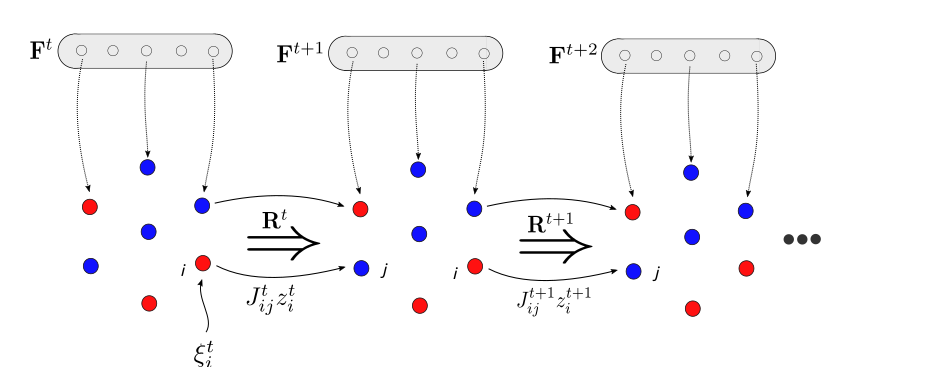
\includegraphics[width=150mm]{figure-1}
\caption{}
\end{figure}


\begin{equation}
\tau\dot{V_{j}}^{\alpha}(t) = -V_{j}^{\alpha}(t) + \zeta_{j}^{\alpha}(t)
\end{equation}

The above equation is a Langevin equation, used frequently in statistical physics. Take the case when $\zeta(t)$ is  the synaptic current arising from excitatory and inhbitory inputs to a neuron in a recurrent spiking network

\begin{align}
\zeta_{j}^{\alpha}(t) = F_{j}^{\alpha}(t) + R_{j}^{\alpha}(t) + \sigma_{j}\sqrt{dt}\eta_{j}^{\alpha}(t)
\end{align}

where we have reserved $\eta(t) \sim \mathcal{N}(0,1)$ for the intrinsic noise of a neuron. We assume that this intrinsic noise is delta correlated i.e. $\langle \eta_{i}(t)\eta_{j}(t)\rangle = \delta(i-j)$ and $\langle \eta_{i}(t)\eta_{i}(t+\tau)\rangle = \delta(\tau)$. In general, the same condition is not necessarily satisifed for the total synaptic current. There are presumably network architectures and stimulus regimes that can realize a case where $\langle \zeta_{i}(t)\zeta_{j}(t)\rangle \neq 0$ and $\langle \zeta_{i}(t)\zeta_{i}(t+\tau)\rangle \neq 0$ for $i \neq j$. However, a natural starting point in the study of excitatory-inhibitory networks is the case where these are indeed zero, on average. If the above condition is not satisfied, synaptic currents will have a ``colored" power spectrum. 

\subsection{Mean-field firing rates in a balanced network}

Local cortical networks can contain thousands of cells, each neuron having thousands of synaptic connections to other cells within the local network as well as other cortical areas (Binzegger 2004). Indeed, connection probabilities between nearby neurons in cortex has been shown experimentally to sometimes exceed 40 percent (Ko 2011; Levy 2012). This small-world feature of cortical networks arguably plays an important role in guiding network dynamics. However, network models that incorporate spatial information present a challenge for theoretical calculations that are simplified when the network contains discrete populations of cells. The random network has been used extensively in the literature, although it has been extended to create a network with a more modular architecture (Sporns 2006). In any case, analytical treatment of network architecture and its relation to dynamics requires a careful definition of the scaling laws of network parameters as a function of network size $N$. Therefore, we begin the theoretical discussion of spiking dynamics by adopting the following terminology for network parameterization. 

\clearpage
\begin{sidewaysfigure}
\centering
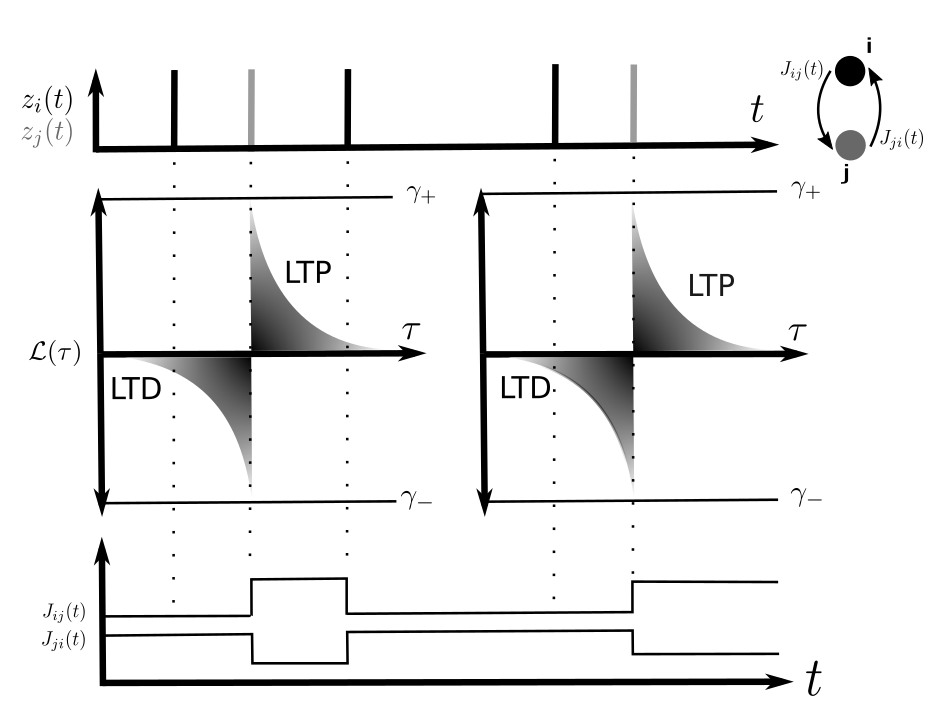
\includegraphics[scale=1.1]{figure-2}
\caption{Weak correlations of synaptic currents in the asychronous state}
\label{fig:foo}
\end{sidewaysfigure}


A network model is called \emph{sparse} if the probability of a connection between arbitrary populations $\alpha$ and $\beta$ scales according to $p_{\alpha\beta} \sim \mathcal{O}(1/N)$ meaning that the degree of a neuron does not depend on the scale of the network or $K \sim \mathcal{O}(1)$. Naturally, we then say that a network is \emph{dense} if the in-degree scales as $p_{\alpha\beta} \sim \mathcal{O}(1)$ such that the degree of a neuron $K \sim \mathcal{O}(N)$. In both of these cases, the strength of a synapse plays an equally important role. The synaptic coupling strength is said to be \emph{strong} if $J^{\alpha\beta} \sim \mathcal{O}(1)$. It is common to define \emph{weak} coupling as the case where $J^{\alpha\beta} \sim \mathcal{O}(1/\sqrt{N})$ such that, when the network is dense, the strength of synaptic connection decreases but at a slower rate than the degree $K$ is increasing. In this case, it is possible that fluctuations in the synaptic input currents saturates to a value of the order of the spiking threshold, in the limit of large networks (Vreeswijk, 1996; Renart 2010; Rosenbaum 2017).

The irregularity of spike timing and large coefficient of variation observed in cortex has presented a challenging puzzle for computational neuroscience. This irregularity results weak but often nonzero correlations in spike trains, raising a number of questions regarding its role in robust sensory processing. Interestingly, this irregular spike timing or \emph{asychronous state} can be reproduced in network simulations via a balance of excitatory and inhibitory synaptic currents (Vreeswijk, 1996). By using a mean-field theory of neuron dynamics, firing rates and spike count correlations can be predicted analytically, for very large networks. In terms of its relationship to network topology, the balanced state can be achieved when synaptic weights are scaled like $J^{\alpha\beta} \sim \mathcal{O}(1/\sqrt{N})$ where $N$ is the network size. The recurrent part of the synaptic current in (3.2) can then be written explicitly giving a total synaptic current

\begin{align}
\xi_{i}^{\alpha}(t) &= F_{i}^{\alpha}(t) + R_{i}^{\alpha}(t) + \eta_{i}(t)\\
&= F_{i}^{\alpha}(t) + \sum_{\beta}\sum_{j} \frac{J_{ij}^{\alpha\beta}}{\sqrt{N}}(\phi * Z^{\beta}_{j}(t)) + \eta_{i}(t)
\end{align}

where the variable $Z^{\beta}_{j}(t) = H(V^{\beta}_{j}(t) - \theta)$ with $H$ being the Heaviside step function. For the sake of generality, the term $\phi * Z^{\beta}_{j}(t)$ represents the convolution of the spike variable $Z^{\beta}_{j}(t)$ with a kernel $\phi$, determining the shape of the post-synaptic current waveform in response to a spike. However, in the remainder of this analysis we will assume that $\phi = \delta(t)$. In the mean-field approximation we replace the individual currents in (3.4) by their average values, which is valid in the limit $N\rightarrow\infty$. This gives the following expression

\begin{align*}
\langle \xi_{i}^{\alpha}(t)\rangle &= \langle F_{i}^{\alpha}(t)\rangle + \langle R_{i}^{\alpha}(t)\rangle + \langle\eta_{i}(t)\rangle\\
&= \langle F_{i}^{\alpha}(t)\rangle + \sqrt{N}\sum_{\beta}J_{\alpha\beta}p_{\alpha\beta}r_{\beta} + \langle\eta_{i}(t)\rangle
\end{align*}

where we have used that $p_{\alpha\beta} = \tilde{p}_{\alpha\beta}p_{\alpha}$ with $\tilde{p}_{\alpha\beta}$ being the probability of a synapse of a neuron $\alpha$ onto type $\beta$ and $p_{\alpha}$ the probability of a neuron being of type $\alpha$. Notice that the average value of the recurrent contribution to the synaptic current saturates for large $N$. Writing the above equation explicitly for a neuron in an excitatory-inhibitory network gives

\begin{align}
\langle \xi_{j}^{e}(t)\rangle &= \langle F_{j}^{e}(t)\rangle + \sqrt{N}\left(j_{ee}p_{ee}r_{e} + j_{ie}p_{ie}r_{i}\right)\\
\langle \xi_{k}^{i}(t)\rangle &= \langle F_{k}^{i}(t)\rangle + \sqrt{N}\left(j_{ii}p_{ii}r_{i} + j_{ei}p_{ei}r_{e}\right)
\end{align}

where subsripts of the from $J_{\alpha\beta}$ refers to the strength of a connection in the direction $\alpha\rightarrow\beta$. If we require that, in the mean-field limit $N\rightarrow\infty$, the external and recurrent currents cancel each other, and $\langle F_{j}^{\alpha}(t)\rangle \sim \mathcal{O}(\sqrt{N})$ we have the following matrix equation

\begin{align}
\begin{pmatrix}
j_{ee} & j_{ie}\\
j_{ei} & j_{ii}
\end{pmatrix}
\begin{pmatrix}
r_{e}\\
r_{i}
\end{pmatrix}
= 
-\begin{pmatrix}
\langle F_{j}^{e}\rangle\\
\langle F_{k}^{i}\rangle
\end{pmatrix}
\end{align}

which can be summarized as $\mathbf{r} = -\mathbf{J}^{-1}\mathbf{f}$. Assuming that $\mathbf{J}$ is invertible, we have the following solution

\begin{align}
\underset{N\rightarrow \infty}{\mathrm{lim}}r_{e} = \frac{\langle F_{j}^{e}\rangle j_{ii}-\langle F_{k}^{i}\rangle j_{ie}}{j_{ei}j_{ie} - j_{ee}j_{ii}}
\end{align}

\begin{align}
\underset{N\rightarrow \infty}{\mathrm{lim}}r_{i} = \frac{\langle F_{k}^{i}\rangle j_{ee}-\langle F_{j}^{e}\rangle j_{ei}}{j_{ei}j_{ie} - j_{ee}j_{ii}}
\end{align}

For positive solutions for the above firing rates and for the above matrix to be invertible we have the condition $\langle F_{j}^{e}\rangle/\langle F_{k}^{i}\rangle > j_{ie}/j_{ii} > j_{ee}/j_{ei}$ and we recover the condition given in (Rosenbaum 2014; Rosenbaum 2017; Akil 2021).



Introducing correlations into synaptic the synaptic currents over a population greatly complicates the development of a solution to (3.7). We can no longer describe the high-dimensional solution with a one-dimensional equation. At the same time, covariance matrices are difficult to predict unless the system satisfies the limit for a mean-field approach. In summary, equation (3.7) must be solved for very large $N$ to avoid finite size effects in a solution of the steady state covariance while nonzero correlations give rise to non-gaussian features.  Of course, traditional numerical methods such as finite element and finite difference all suffer from the curse of dimension (Chen 2017, Pichler 2013). Another solution is a Monte Carlo simulation of (X); however, the required sample size increases in an exponential rate as the dimension and the same curse dimensionality problem appears. However, recently a method for solving the Fokker-Planck equation in high dimensions, even on the order of millions, has been developed for complex systems with non-gaussian features (Chen 2017). 

The following model for generating the backbone for network of neurons rests on the assumption that we can create connectivity solely from pairwise connection probabilities. Let us define a spatial connectivity kernel $\Gamma_{i}(\mathbf{r}_{j})$ with $i,j\in \{n\}_{n=1}^{N}$ which defines the binomial probability that a neuron $i$ synapses onto a different cell $j\neq i$ at spatial coordinate $\mathbf{r}_{j}$. Here, the function $\Gamma_{i}(\mathbf{r})$ is not itself a probability distribution but rather represents one component of a distribution that is defined for each possible pairs $i,j$ for a given $i$. That distribution is completely represented for a pair $i,j$ with knowledge of the kernel $\Gamma_{j}(\mathbf{r}_{i})$ and an additional probability that no synapse occurs $\Gamma_{0}$. The parameter $\Gamma_{0}$ will be referred to as the $\emph{sparsity parameter}$ throughout the remainder of the text. Together, these three binomial probabilities can be renormalized to form a multinomial distribution $\mathbb{P}_{ij}$ at every possible synapse $ij$. A general definition of the multinomial distribution is

\begin{align}
\mathbb{P} = \frac{p_{n}\prod_{m\neq n}(1-p_{m})}{\sum_{n}p_{n}\prod_{m\neq n}(1-p_{m})} = \frac{p_{n}\prod_{m\neq n}(1-p_{m})}{Z}
\end{align}

where $Z$ is a normalization constant. For generating synapses, the probabilities of (3.1) are the probabilities over the possible synaptic states between $i$ and $j$

\begin{equation}
    \mathbb{P} = \left\{\begin{array}{lr}
        p_{ij} = \Gamma_{ij}(1-\Gamma_{ji})(1-\Gamma_{0})\cdot Z^{-1}\\
        p_{ji} = \Gamma_{ji}(1-\Gamma_{ij})(1-\Gamma_{0})\cdot Z^{-1}\\
        p_{0} = \Gamma_{0}(1-\Gamma_{ij})(1-\Gamma_{ji})\cdot Z^{-1}\\
        \end{array}\right\}
\end{equation}
  
\begin{align*}
Z = \Gamma_{ij}(1-\Gamma_{ji})(1-\Gamma_{0}) + \Gamma_{ji}(1-\Gamma_{ij})(1-\Gamma_{0}) + \Gamma_{0}(1-\Gamma_{ij})(1-\Gamma_{ji})
\end{align*}

Sampling from the distribution $\mathbb{P}$ for each of the $N^{2} - N$ possible synapses (excluding autapses), we can generate an asymmetric adjacency matrix $\mathcal{C} \in \mathbb{F}_{2}^{N\times N}$. An element $\mathcal{C}_{ij} = 1$ defines a synapse from $i\rightarrow j$ and $\mathcal{C}_{ji} = 1$ defines a synapse from $j\rightarrow i$.

Defining the generation of network connectivity in this way proves useful upon the realization that the network can be described by binomial statistics, similar to the well-known Erdos-Renyi (ER) random graph. Graph theory provides a rich set of metrics that can be used to discuss the statistical properties of the network defined by $\mathcal{C}$ and in turn the chosen kernel $\Gamma$. Assuming that we can compute the probabilities $p_{ij}, p_{ji}$ and $p_{0}$ for a particular $\Gamma$ and every synapse is generated independently, the mean of the out-degree distribution is

\begin{equation}
\langle N_{ij} \rangle = \sum_{j} \Gamma_{ij}(1-\Gamma_{ji})(1-\Gamma_{0})\cdot Z^{-1}
\end{equation}

where the spatial dependence of the individual kernels is implied. The in-degree distribution is found by simply swapping $i$ and $j$. The variance of the out-degree distribution is then

\begin{align}
\mathrm{Var}(N_{ij}) &= \sum_{j} \langle N_{ij}^{2} \rangle - \langle N_{ij} \rangle ^{2} \\
&= \sum_{j} \langle N_{ij}\rangle - \langle N_{ij} \rangle ^{2} 
\end{align}

from the linearity of variance property. We will analyze the in-degree and out-degree distributions of a graph generated when the connectivity kernel is a symmetric Gaussian extending over two-dimensions. We refer to this case as a \emph{two-dimensional gaussian network}.


\subsection{The two-dimensional Gaussian network}

Suppose that we have a two-dimensional lattice which contains points separated by a distance $\Delta$ along the axial directions with periodic boundary conditions. The distance between any two points on such a lattice is the following Euclidean distance metric

\begin{align*}
|\Delta\mathbf{r}_{ij}|^{2} = \mathrm{min}(|x_1 - x_2|, n\Delta - |x_1 - x_2|)^2 + \mathrm{min}(|y_1 - y_2|, n\Delta - |y_1 - y_2|)^2
\end{align*}

Now, let the kernel $\Gamma_{ij}$ be the two-dimensional symmetric Gaussian

\begin{align}
\Gamma_{ij}(|\Delta\mathbf{r}_{ij}|) = \gamma\cdot \exp\left(-\frac{1}{2}(\mathbf{r}_{i}-\mathbf{r}_{j})^{T}\mathbf{\Sigma}_{i}(\mathbf{r}_{i}-\mathbf{r}_{j})\right)
\end{align}

where $\mathbf{\Sigma}_{i} = \sigma_{i}^{2}I$ with the two-dimesional identity matrix $I$. The parameter $\sigma_{i}$ can be intepreted as the \emph{reach} of a neuron $i$. Furthermore, for the kernel $\Gamma_{ij}$ to represent a binomial probability at each point of its domain, we must have that


\begin{equation}
\Gamma_{ij}(|\Delta\mathbf{r}_{ij}|)  \leq 1
\end{equation}

Plugging in our definition (3.5) gives the following inequality

\begin{align*}
\gamma\cdot \exp\left(-\frac{\underset{j}{\mathrm{min}}\left(|\Delta\mathbf{r}_{ij}|^{2}\right)}{2\sigma_{i}^{2}} \right) \leq 1
\end{align*}

The largest possible value of the exponential is achieved at $\underset{j}{\mathrm{min}}\left(|\Delta\mathbf{r}_{ij}|^{2}\right) = \Delta$ (a neighboring lattice point). Therefore, $\gamma$ is upper bounded according to $\gamma \leq \exp\left(\frac{\Delta^{2}}{2\sigma_{i}^{2}}\right)$. For the remainder of our analysis we will fix $\gamma = 1$ and focus our attention to the impact of the parameters $\sigma$ and $\Gamma_{0}$ on the statistics of connectivity. 

As can be seen in Fig. (3.1a), when $\Gamma_{ij} = \Gamma_{ji}$ we have that $p_{ij} = p_{ji}$ for all $|\Delta \mathbf{r}_{ij}|$. We formally refer to this case as the \emph{homogeneous gaussian network}. While this is not necessarily a realistic case, it serves as a useful testbed for the graph theoretic concepts to be used in later analyses. 

\clearpage
\begin{figure}[t!]
\centering
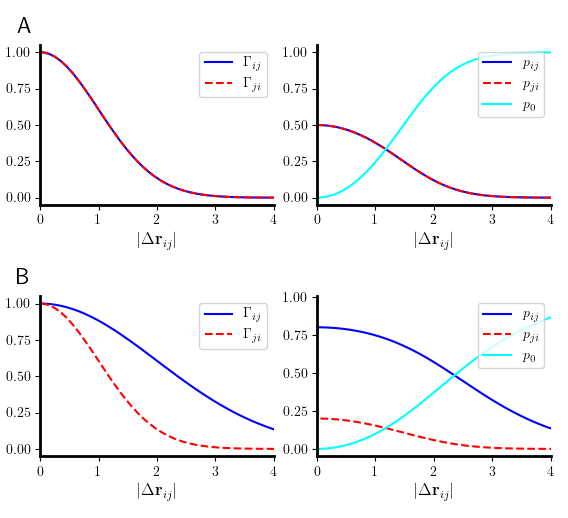
\includegraphics[width=100mm]{fig_11}
\caption{\textbf{Synapse probabilities for gaussian connectivity} (a) Binomial probabilities for two identical gaussian kernels ($\sigma=1$) separated by a distance $|\Delta\mathbf{r}_{ij}|$ and the probability of no synapse $\Gamma_{0}$ (left) and the corresponding multinomial probabilities (right). (b) Binomial probabilities for two different gaussian kernels ($\sigma_{1}=1, \sigma_{2}=2$) separated by a distance $|\Delta\mathbf{r}_{ij}|$ and the probability of no synapse $\Gamma_{0}$ (left) and the corresponding multinomial probabilities (right). }
\end{figure}



\subsection{Homogeneous Gaussian networks}

Let us now examine the statistics of the out-degree of a neuron $i$ assuming that the connectivity parameter $\sigma$ and $\Gamma_{0}$ are homogeneous across the network i.e., they are constant for all neurons. Using Eq. (3.2), we have

\begin{align}
\langle N_{ij} \rangle &= \left(\frac{1-\Gamma_{0}}{N}\right)\sum_{j} \Gamma_{ij}(1-\Gamma_{ji})\cdot Z_{ij}^{-1}
\end{align}

a sum that can be carried out numerically. Interestingly, in the homogeneous case, the parameter $\gamma$ and $\Gamma_{0}$ become redundant. This can be seen by considering that multiplying $p_{ij}$ and $p_{ji}$ by the same constant factor $\gamma$ is equivalent to the transformation $\Gamma_{0}' = 1-\gamma(1-\Gamma_{0})$. 

\clearpage
\begin{figure}[t!]
\centering
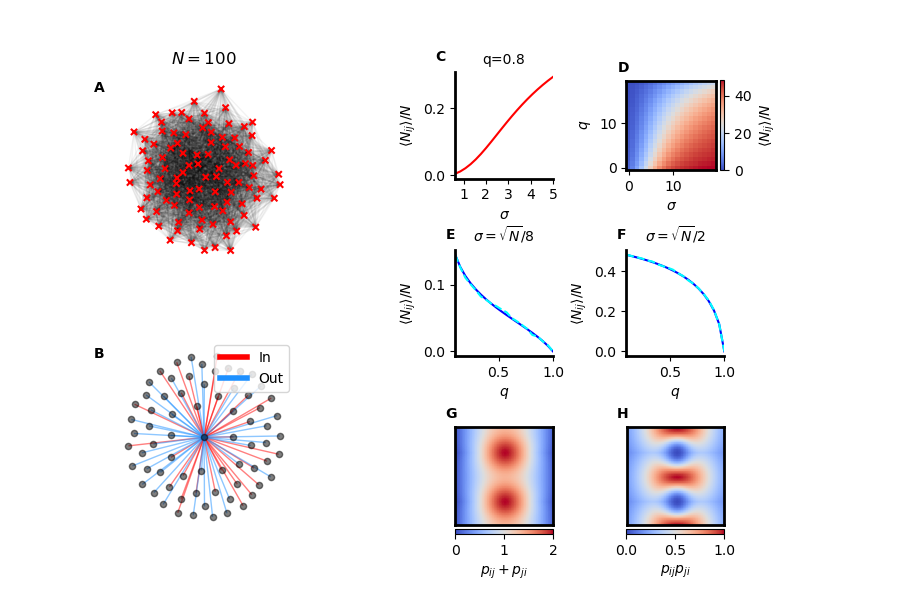
\includegraphics[width=175mm]{fig_8}
\caption{\textbf{The homogeneous Gaussian network}. (A) An example homogeneous network containing $N=100$ neurons. (B) An example neuron extracted from (A) with outgoing synapses labeled in blue and incoming synapses labeled in red. (C,D) The ratio $\langle N_{ij}\rangle/N$ as a function parameters ($\sigma, \Gamma_{0}$) for a sparse network (C) and a network with variable sparsity (D). (E,F) The ratio $\langle N_{ij}\rangle/N$ for fixed $\sigma$ and variable sparsity. (G,H) Binomial probability maps for two nearby neurons expressed as a sum $p_{ij}+p_{ji}$ and product $p_{ij}p_{ji}$}
\end{figure}

In other words, for the homogeneous case, the multiplication by $\gamma$ can be represented by a suitable selection of $\Gamma_{0}$ and can be set $\gamma=1$. Numerical evaluation of (3.7) shows that the ratio $\langle N_{ij}\rangle$ increases monotonically for increasing $\sigma$, as expected from (3.1b) and saturates at $\langle N_{ij}\rangle = 0.5$ at a rate proportional to $\sigma$. This can be understood from the fact that as $\Gamma_{0} \rightarrow 1$ we have $p_{0} \rightarrow 0$ and the multinomial distribution in (3.2) is reduced to a binomial distribution with $p_{ij} = p_{ji} = 1/2$. 

Furthermore, in addition to the average degree of a neuron, we are interested in the average number of shared inputs (outputs) between two neurons. We expect that this statistic makes at least a partial contribution to pairwise correlations in the voltage dynamics between two cells. To address this, we consider the average number of shared connections $\langle S_{ij} \rangle$ between a neuron $i$ and $j$ as a function of their distance $|\Delta \mathbf{r}_{ij}|$. In essence, this is the product $p_{ik}\cdot p_{jk}$ for a third neuron $k$ with $i,j\neq k$. The symmetry present in the homogeneous case allows us to perform this computation rather easily,

\begin{align}
\langle S_{ij} \rangle &= \frac{1}{N}\sum_{k} p_{ik}\cdot p_{jk} \\
&= \frac{\left(1-\Gamma_{0}\right)^{2}}{N}\sum_{k}\frac{\Gamma_{ik}(1-\Gamma_{ki})\Gamma_{jk}(1-\Gamma_{kj})}{Z_{ik}Z_{jk}}
\end{align}


which can be carried out numerically over the two-dimensions of space. Self-consistent with our definition of the connectivity kernel, the normalized number of shared connections decays with a gaussian profile for increasing $|\Delta \mathbf{r}_{ij}|$ as can be seen in Fig. (3.3).
\begin{figure}
\centering
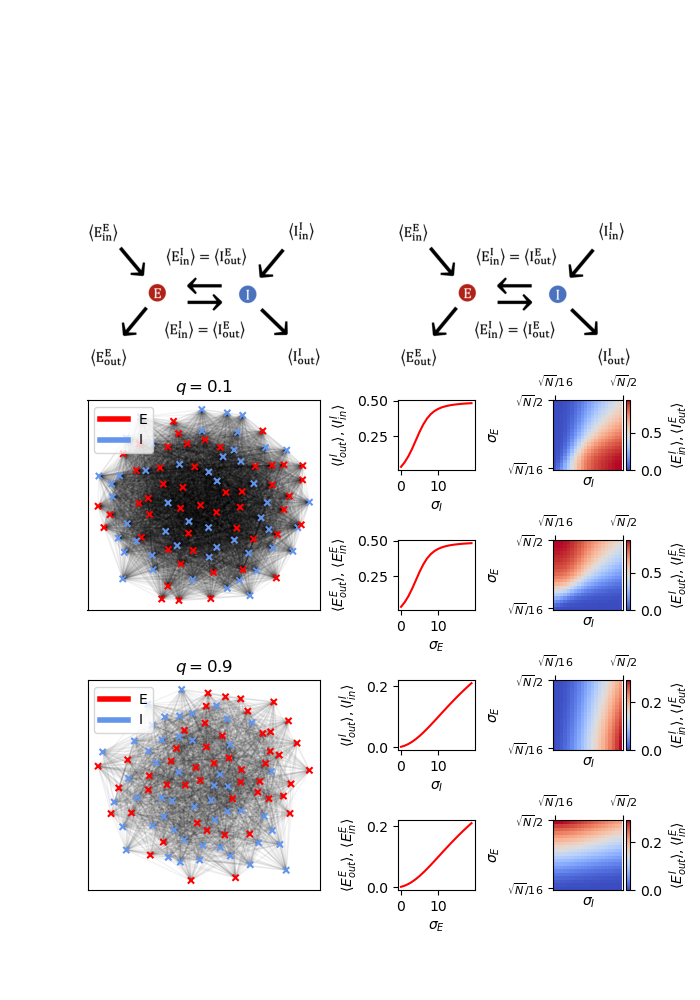
\includegraphics[width=175mm]{fig_9}
\caption{\textbf{Shared connections in a homogeneous Gaussian network} (A,B,C) The average number of shared incoming or outgoing connections $\langle S_{ij}\rangle /N$ as a function of distance between two neurons $|\Delta r_{ij}|$ for three different values of the reach parameter $\sigma$.}
\end{figure}

\clearpage



\subsection{Excitatory-inhibitory Gaussian networks}

Thus far we have considered only the case where the spatial connectivity kernel is the same for every neuron. However, the integrative properties of neurons depend strongly on the number, proportions and distribution of excitatory and inhibitory synaptic inputs they receive (Megias 2001). Also, the role excitatory-inhibitory balance in network dynamics has been a subject of recent debate. Indeed, balanced recurrent excitation and inhibition capture the irregular and asynchronous spiking activity with weak correlations reported in cortex. The spatial extent of excitation relative to inhibition has been shown to have a strong impact on network dynamics. In particular, when the spatial extent of excitation is sufficiently smaller than inhibition, the balanced fixed point loses stability (Rosenbaum 2014). 

To account for excitatory and inhibitory cell types within this framework, we must differentiate $\langle N_{ij}\rangle$ for excitatory and inhibitory neurons and solving for both the mean in-degree and out-degree separately. Thus we have the quantities $\langle E_{E}^{\mathrm{out}} \rangle,\langle E_{I}^{\mathrm{out}} \rangle,\langle E_{I}^{\mathrm{in}} \rangle$ and $\langle I_{E}^{\mathrm{out}} \rangle,\langle I_{I}^{\mathrm{out}} \rangle,\langle I_{E}^{\mathrm{in}} \rangle$. Under the assumption that excitatory and inhibitory neurons are distributed uniformly  in two-dimensional space, we have that $\langle E_{I}^{\mathrm{out}} \rangle = \langle I_{E}^{\mathrm{in}} \rangle$ and $\langle E_{I}^{\mathrm{in}} \rangle = \langle I_{E}^{\mathrm{out}}\rangle$. For brevity, we drop the superscripts and compute the above averages according the general prescription provided by (3.3). The result of these numerical calculations allow us to observe that, for $\Gamma_{0} = 0.2$, the fraction of the target population saturated by excitatory or inhibitory outputs increases monotonically with $\sigma_{E}$ and $\sigma_{I}$  (Fig 3.4 b,d). The parameter maps provided in (Fig 3.4 b,d) are a starting point for our later discussions of newtork dynamics. 


\clearpage
\begin{figure}[t!]
\centering
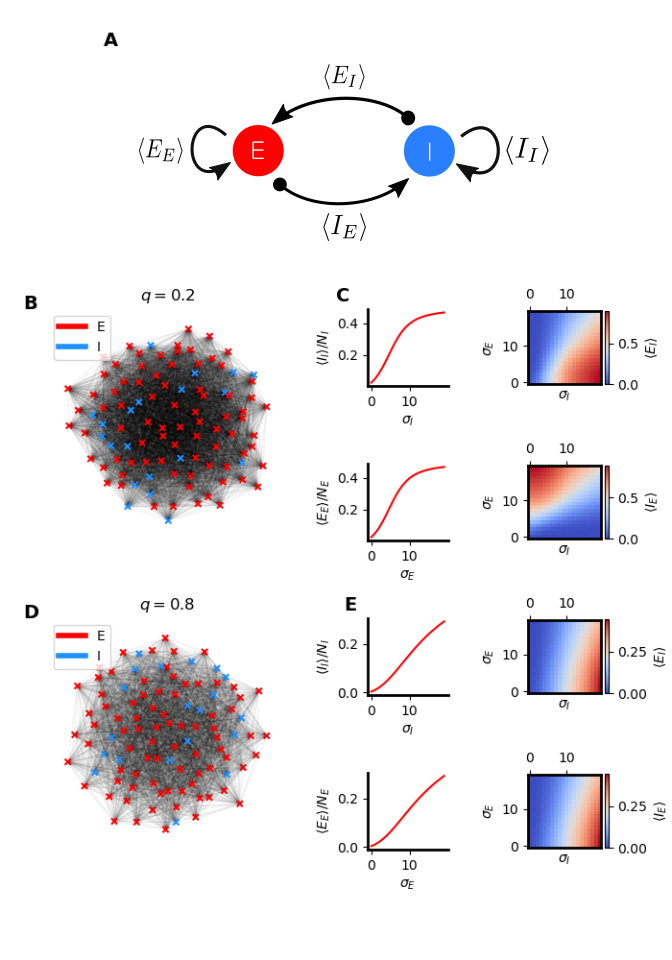
\includegraphics[width=165mm]{fig_10}
\caption{\textbf{Average degree in an excitatory-inhibitory network} (A) Schematic illustrating the notation used for excitatory-excitatory, excitatory-inhibitory, inhibitory-excitatory, and inhibitory-inhibitory synapses. (B) An example dense excitatory-inihbitory network ($\Gamma_{0}=0.2$) and $p_{E} = 0.8$. (C) Average number of synapses in the dense network normalized to the target population size as a function of parameters $\sigma_{E}$ and $\sigma_{I}$. (D) An example sparse excitatory-inihbitory network ($\Gamma_{0}=0.8$) and $p_{E} = 0.8$. (E) Average number of synapses in the sparse network normalized to the target population size as a function of parameters $\sigma_{E}$ and $\sigma_{I}$.}
\end{figure}


\section{Methods}

\subsection{Signal processing techniques}

The cross-correlation of discrete signals $x(t)$ and $y(t)$ is generally defined as the following convolution in the time-domain

\begin{align}
R_{xy}(\tau) = x(t) * y(t) = \sum_{k =-\infty}^{\infty}x(t)y(t+\tau)
\end{align}

where the $*$ symbol represents the convolution operation. Let $\psi_{x}(\omega)$ be the discrete-time Fourier transform (DTFT) of $x(t)$ i.e.,

\begin{align}
\psi_{x}(\omega) = \sum_{t =-\infty}^{\infty}x(t)\left(\exp{-i\omega t}\right)
\end{align}

where an identical expression exists for $\psi_{y}(\omega)$. According to the convolution theorem, convolution in the time-domain is equivalent to multiplication in the frequency domain with one of the signals time-reversed. Therefore, we can write

\begin{align}
\mathrm{DTFT}[x(t) * y(t)](\omega) = \underset{T\rightarrow\infty}{\mathrm{lim}}\frac{1}{2\pi T}\psi_{x}^{*}(\omega)\psi_{y}(\omega)
\end{align}


Let $S_{xy}(\omega) = \underset{T\rightarrow\infty}{\mathrm{lim}}\frac{1}{2\pi T}\psi_{x}^{*}(\omega)\psi_{y}(\omega)$, which is commonly called the \emph{cross spectral density} of signals $x(t)$ and $y(t)$. This is simply the DTFT of the cross-correlation function meaning that $R_{xx}(\tau)$ and $S_{xx}(\omega)$ form a Fourier pair. This result provides us an efficient means of computing cross-correlations and autocorrelations of synaptic currents by multiplication in the frequency domain and taking the inverse discrete transform.

 After enforcing the boundary conditions appropriate for a neuron with a threshold $\theta$ and a nonzero refractory period $\tau_{\mathrm{ref}}$, we arrive at a steady state solution for the instantaneous firing rate (Brunel 2000). 

\begin{align}
\frac{1}{\nu_{0}} = \tau_{\mathrm{ref}} + \tau\sqrt{\pi}\int_{\frac{V_{r}-\mu_{0}}{\sigma_{0}}}^{\frac{\theta-\mu_{0}}{\sigma_{0}}} \exp(u^{2})(1+\mathrm{erf}(u))du
\end{align}

and previous solutions to (3.1) do not apply (Brunel 2000). In the worst case, the one-dimensional Fokker-Planck equation must be solved in $N$ dimensions and the covariance matrix of synaptic currents must be known. For the $N$ dimensional case, (3.1) generalizes to 

\begin{equation}
\tau\dot{\mathbf{V}}(t) = -\mathbf{V}(t) + \mathbf{\Sigma}(t)\mathbf{W}(t)
\end{equation}

For arbitrary connectivity patterns, estimating the systems covariance is challenging, although the problem was recently addressed via a mean-field theory for discrete networks and networks with spatial connectivity (Rosenbaum 2017). We now summarize the Kramers-Moyal expansion, a full derivation is included in (A.1). followed by a short summary of this mean-field theory.

The problem at hand is the determination of the distribution of the state variable $V$ for a neuron $j$ i.e. the density $P_{j}(V)$ as a function of time. The central assumption made in the derivation of the Kramers-Moyal expansion is that the evolution of $P_{j}(V_{j},t)$ follows a Markov chain. We are then permitted to write the Chapman-Kolmogorov (CK) equation

\begin{equation}
P(V'_{j}, t) = \int T_{j}(V'_{j}, t | V_{j}, t-\tau)P(V_{j}, t-\tau)dV
\end{equation} 

which expresses the density of $V$ in terms of an integral over a transition density $T_{j}$. The transition density is directly related to the distribution over synaptic currents. If $T_{j}$ is normally distributed, then $P(V_{j},t)$ must also be normally distribution (as in the Ornstein-Uhlenbeck process). Starting from the CK equation in (1.3) we can derive the Kramers-Moyal Expansion (KME) which has the form

\begin{align}
\frac{\partial P_{j}}{\partial t} = \sum_{n} \frac{(-1)^{n}}{n!} \left(\frac{\partial}{\partial V_{j}}\right)^{n} M_{n}(V_{j},t,\tau) P(V_{j},t)
\end{align}

where $M_{n}(V,t,\tau)$ denotes the $nth$ order moment of the transition density $T_{j}(V'_{j}, t | V_{j}, t-\tau)$. If we approzetamate the KME by truncating the summation for $n > 2$ we arrive at the so-called \emph{diffusion approzetamation} or Fokker-Planck equation

\begin{align}
\frac{\partial P_{j}}{\partial t} &= \frac{\partial}{\partial V_{j}}[\left(V_{j}(t)-\mu_{j}(t)\right) P_{j}(V_{j},t)] + \frac{\sigma_{j}^{2}(t)}{2}\frac{\partial^{2}}{\partial V_{j}^{2}}[P(V_{j},t)]
\end{align}

where the first and second moments have been substituted by their standard symbols $\mu$ and $\sigma^{2}$. The general form of the Fokker-Planck equation in $N$ dimensions; that is, the time-dependence of the joint distribution over $N$ voltage variables $P(V_{1}\;...\;V_{N})$ is

\begin{align}
\frac{\partial P}{\partial t} &= \sum_{i}
\beta_{ij}\frac{\partial}{\partial V_{i}}[\left(V_{j}(t)-\mu_{j}(t)\right) P_{j}(V_{j},t)] + \sum_{i}D_{ij}\frac{\partial^{2}}{\partial V_{i}\partial V_{j}}[P(V_{j},t)]
\end{align}

where the term $D_{ij}$ is called the \emph{diffusion tensor} and is related to the covariance matrix $\Sigma$ by $D_{ij} = \frac{\Sigma\Sigma^{T}}{2}$.


\begin{appendices}
\chapter{The Kramers-Moyal expansion}

Given many instantiations of a stochastic variable $V$, we can construct a normalize histogram over all observations as a function of time $P(V,t)$. However, in order to systematically explore the relationship between the parameterization of the process and $P(V,t)$ we require an expression for $\dot{P}(V,t)$. If we make a fundamental assumption that the evolution of $P(V,t)$ follows a Markov process i.e. its evolution has the memoryless property, then we can write

\begin{equation}
P(V', t) = \int T(V', t | V, t-\tau)P(V, t-\tau)dV
\end{equation} 

which is known at the Chapman-Kolmogorov equation. The factor $T(V', t | V, t-\tau)$ is known as the \emph{transition operator} in a Markov process and determines the evolution of $P(V,t)$ in time. We proceed by writing $T(V', t | V, t-\tau)$ in a form referred to as the Kramers-Moyal expansion

\begin{align*}
T(V', t | V, t-\tau) &= \int \delta(u-V')T(u, t | V, t-\tau)du\\
&= \int \delta(V+u-V'-V)T(u, t | V, t-\tau)du\\
\end{align*} 

If we use the Taylor expansion of the $\delta$-function 

\begin{equation*}
\delta(V+u-V'-V) = \sum_{n=0}^{\infty} \frac{(u-V)^{n}}{n!}\left(-\frac{\partial}{\partial V}\right)^{n}\delta(V-V')
\end{equation*}

Inserting this into the result from above, pulling out terms independent of $u$ and swapping the order of the sum and integration gives

\begin{align}
T(V', t | V, t-\tau) &= \sum_{n=0}^{\infty} \frac{1}{n!}\left(-\frac{\partial}{\partial V}\right)^{n}\delta(V-V')\int(u-V)^{n}T(u, t | V, t-\tau)du\\
&= \sum_{n=0}^{\infty} \frac{1}{n!}\left(-\frac{\partial}{\partial V}\right)^{n}\delta(V-V')M_{n}(V,t)
\end{align} 

noticing that $M_{n}(V,t) = \int(u-V)^{n}T(u, t | V, t-\tau)du$ is just the $n$th moment of the transition operator $T$. Plugging (2.6) back in to (2.4) gives 

\begin{align}
P(V, t) &= \int \left(1 + \sum_{n=1}^{\infty} \frac{1}{n!}\left(-\frac{\partial}{\partial V}\right)^{n} M_{n}(V,t)\right)\delta(V-V')P(V, t-\tau)dV\\
&= P(V', t-\tau) + \sum_{n=1}^{\infty} \frac{1}{n!}\left(-\frac{\partial}{\partial V}\right)^{n} \left[M_{n}(V,t)P(V,t)\right]
\end{align} 

Approzetamating the derivative as a finite difference and taking the limit $\tau\rightarrow 0$ gives

\begin{align}
\dot{P}(V,t)  &= \underset{\tau\rightarrow 0}{\mathrm{lim}}\left(\frac{P(V, t)-P(V, t-\tau)}{\tau}\right)\\
&= \sum_{n=1}^{\infty} \frac{1}{n!}\left(-\frac{\partial}{\partial V}\right)^{n} \left[M_{n}(V,t)P(V,t)\right]
\end{align} 

which is formally known as the Kramers-Moyal (KM) expansion. The Fokker-Planck equation is a special case of (2.10) where we neglect terms $n>2$ in the \emph{diffusion appromation}.
\end{appendices}

% Format a LaTeX bibliography
\makebibliography

[1] D.O. Hebb \textit{The organization of behavior: A neurophysiological theory}. John Wiley and Sons. 1949.

% Figures and tables, if you decide to leave them to the end
%\input{figure}
%\input{table}

\end{document}


